\documentclass[10pt,oneside]{article}

\usepackage[T1]{fontenc}

\usepackage[paper=a4paper,margin=2cm,bottom=2.5cm]{geometry}
\usepackage[sfdefault,light,condensed]{roboto}
\usepackage[export]{adjustbox}
\usepackage[usenames,dvipsnames,table]{xcolor}

\usepackage{amsmath,amssymb,array,fancyhdr,graphicx,enumitem,lastpage,listings,lstautogobble,multicol,tabularx,textcomp,titlesec}
\usepackage{mathtools}

\setlength\parindent{0cm}
\renewcommand\headrule{}
\setlength{\footskip}{1.25cm}


\pagestyle{fancy}

\usepackage{fontawesome,subcaption,tikzsymbols}

% Add some padding to all table cells.
\setlength\extrarowheight{1pt}

%\newcommand{\boxwidth}{\dimexpr\linewidth - 2pt}
\newcommand{\boxwidth}{\linewidth}

\definecolor{BoxHeaderBG}{RGB}{50, 50, 50}
\definecolor{BoxHeaderText}{RGB}{220, 220, 220}

\definecolor{QuestionHeaderBG}{RGB}{200, 200, 200}
\definecolor{QuestionHeaderText}{RGB}{0, 0, 0}

\newcommand{\BoxHeader}[2]{
    \multicolumn{#1}{| >{\bfseries\footnotesize\cellcolor{BoxHeaderBG}\arraybackslash}l |}{
        \textcolor{BoxHeaderText}{#2}
    }
}

\newcounter{QuestionCounter}

\newcommand{\Question}[2]{
    \stepcounter{QuestionCounter}
    \begin{tabularx}{\boxwidth}{|X|}
        \hline
        \cellcolor{QuestionHeaderBG}{\footnotesize\bfseries \textcolor{QuestionHeaderText}{Question \#\theQuestionCounter}} {\em \textcolor{QuestionHeaderText}{#1}} \\\hline
        \ \\[#2]\hline
    \end{tabularx}

    \medskip
}

\newcommand{\FeelQuestion}{
    \stepcounter{QuestionCounter}
    \newcolumntype{F}{>{\centering\arraybackslash}X}
    \begin{tabularx}{\boxwidth}{| F F F |}
        \hline
        \multicolumn{3}{| >{\hsize=\dimexpr3\hsize+4\tabcolsep+2\arrayrulewidth\relax}X |}{
            \cellcolor{QuestionHeaderBG}{\footnotesize\bfseries \textcolor{QuestionHeaderText}{Question \#\theQuestionCounter}} {\em \textcolor{QuestionHeaderText}{Select the option which best reflects how confident you are in applying what you have learend in this lesson.}}}\\\hline
        & & \\[-8pt]
        \Sadey[5][orange] & \Neutrey[5][gray] & \Smiley[5][cyan] \\\hline
    \end{tabularx}

    \medskip
}

\lhead{\tiny\texttt{U\UnitNumber: \UnitTitle\\L\LessonNumber: \LessonTitle}}
\rhead{\tiny\texttt{[DPCS/\CourseLevel/U\UnitNumber/\LessonNumber]\\ }}

\lfoot{
\includegraphics[height=2cm,valign=c]{Files/logo}}
\cfoot{\footnotesize \LessonTitle/DPCS/\CourseLevel/U\UnitNumber/L\LessonNumber/\thepage/\pageref{LastPage}\\Woodstock School/Mussoorie, Uttarakhand, India}
\rfoot{
\includegraphics[height=2cm,valign=c]{Files/ib-world-school-logo-1-colour}}


\def\CourseLevel{LL}

\def\UnitNumber{01}
\def\UnitTitle{The Computer}

\def\LessonNumber{04}
\def\LessonTitle{The Operating System}

\begin{document}
    %Lesson Title
    \begin{center}
        \Large\bfseries \LessonTitle
    \end{center}

    % Objectives List
    \begin{tabularx}{\boxwidth}{|>{\small\raggedleft\bfseries\arraybackslash}p{0.1\textwidth} >{\small\arraybackslash}X |}
        \hline
        \BoxHeader{2}{Objective} \\\hline
        2.1.6 & Describe the main functions of an operating system. \\\hline
    \end{tabularx}

    % Opening Exercise
    \section*{Before You Begin}
    The following image shows the sound setup for an old MS-DOS game (``Nascar Racing'') using the DOSBox  emulator software.

    \begin{figure}[h]
        \centering
        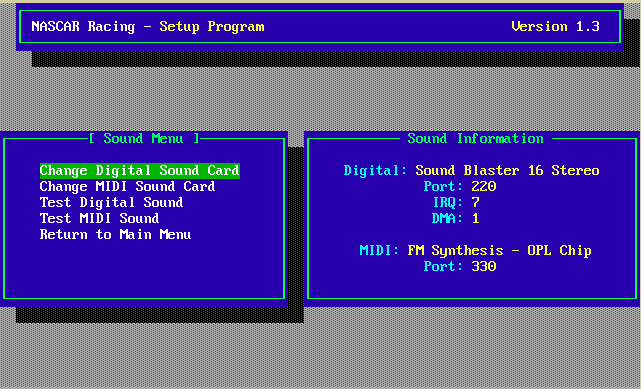
\includegraphics[height=7cm]{Extras/hardware_details}
        \caption*{\tiny Image courtesy abandonia.com.}
        \caption{A screenshot of ``Nascar Racing'' showing user manipulation of the sound card.}
    \end{figure}

    In particualr, note the level of detail about the system sound card the game requires in order to function properly.

    \vfill

    \Question{Modern operating systems provide abstraction through device drivers and system libraries for interacting with common system hardware and peripherals (such as sound board, graphic cards, input devices, etc.). How does this abstraction layer impact the development of software on these systems?}{3.25cm}

    \Question{The typical user of a computer system does not need to interact directly with his/her hardware; however, many games benefit from game-specific settings which impact performance and gameplay. How important is it for the user of a computer system to be able to manipulate some aspects of their hardware directly?}{3.25cm}
    \pagebreak
    
    % Definitions
    \section*{Important Terms}
    \begin{tabularx}{\boxwidth}{| >{\bfseries\arraybackslash}p{0.3\textwidth} | X | }
        \hline
        \BoxHeader{1}{Term} & \BoxHeader{1}{Definition} \\\hline
        Device Driver & \\[2cm]\hline
        Hardware Abstraction Layer & \\[2cm]\hline
        Kernel & \\[2cm]\hline
        Kernel Space & \\[2cm]\hline
        Operating System (OS) & \\[2cm]\hline
        User Space & \\[2cm]\hline
    \end{tabularx}

    \pagebreak

    % Technical Background
    \section*{Technical Background}

    \subsection*{The Role of the Operating System}
    The following diagram is an abstraction showing where the operating system exists in relation to the user applications and the system hardware.

    \medskip
    \begin{figure}[h]
        \centering
        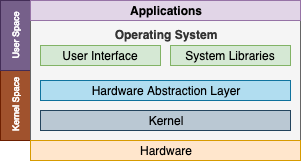
\includegraphics[width=8cm]{Extras/operating_system_simple}
        \caption{A simple view of the software layers of a computer system.}
    \end{figure}

    \subsubsection*{Notes}

    \vfill

    \Question{What benefit does the segregation of memory space for core kernel operations from user-initiated operations have on the stability of a computer system? Are there any drawbacks to this model?}{4cm}

    \pagebreak

    \subsection*{Monolithic vs. Microkernel Operating Systems}

    The following two diagrams show a sample of fundamental services offered by the operating system, and where they would exist within a monolithic or microkernel operating system architecture.

    \medskip
    \begin{figure}[h]
        \centering
        \begin{subfigure}{0.45\boxwidth}
            \centering
            \caption*{\bfseries Monolithic}
            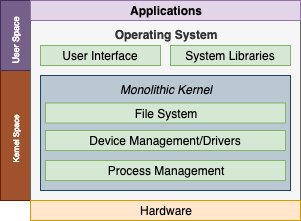
\includegraphics[width=6cm]{Extras/operating_system_monolithic}
        \end{subfigure}
        \begin{subfigure}{0.45\boxwidth}
            \centering
            \caption*{\bfseries Microkernel}
            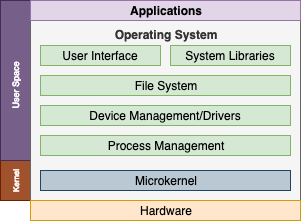
\includegraphics[width=6cm]{Extras/operating_system_microkernel}
        \end{subfigure}
        \caption{Monolithic vs. Microkernel Architectures.}
    \end{figure}
    
    \subsubsection*{Notes}

    \vfill

    \Question{Monolithic kernels run a higher risk of instability due to all services being included in a single process. Despite this, operating systems which are considered \emph{more stable} and \emph{more secure}, such as Linux, generally use monolithic kernels, while systems considered \emph{less stable} and \emph{less secure}, such as Mac OSX and Windows, use microkernels. Why do you think this contradiction exists?}{4cm}

    \pagebreak
    % Developing Technical Skills
    \section*{Developing Technical Skills}
    \subsubsection*{Kernel Development}
    As an open-source project, the Linux kernel grants us the opportunity to examine the kernel development process. In particular, we can note that the kernel has to be created in such a way as to handle the wide variety of hardware platforms now available on the market.

    \medskip
    The following excerpt is taken from the changelogs for version 5.3.12 of the Linux kernel:

    {\footnotesize
    \begin{verbatim}
    Author: Kai-Heng Feng <kai.heng.feng@canonical.com>
    Date:   Wed Oct 16 18:38:16 2019 +0800
    
        x86/quirks: Disable HPET on Intel Coffe Lake platforms
        
        commit fc5db58539b49351e76f19817ed1102bf7c712d0 upstream.
        
        Some Coffee Lake platforms have a skewed HPET timer once the SoCs entered
        PC10, which in consequence marks TSC as unstable because HPET is used as
        watchdog clocksource for TSC.
        
        Harry Pan tried to work around it in the clocksource watchdog code [1]
        thereby creating a circular dependency between HPET and TSC. This also
        ignores the fact, that HPET is not only unsuitable as watchdog clocksource
        on these systems, it becomes unusable in general.
        
        Disable HPET on affected platforms.
    \end{verbatim}
    }

    Navigate to https://www.kernel.org and select the changelog link for the most current \emph{stable} release.

    \begin{figure}[h]
        \centering
        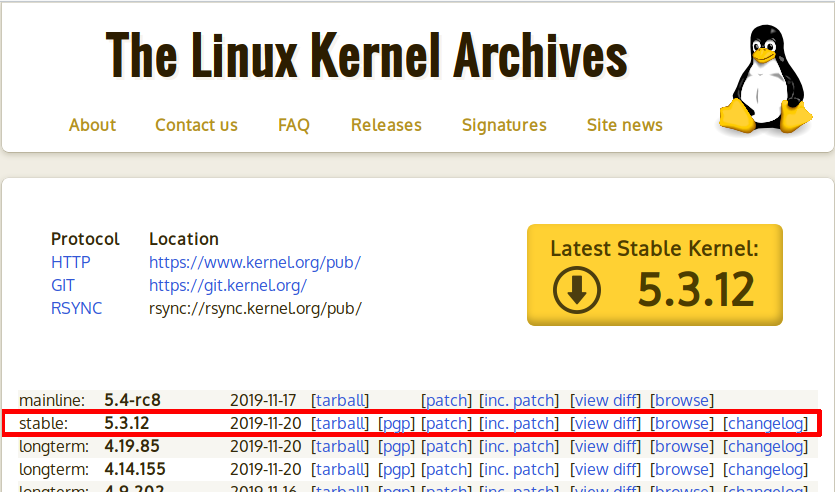
\includegraphics[width=0.5\boxwidth]{Extras/linux_kernel}
        \caption{Screenshot of the Linux Kernel Archives.}
    \end{figure}

    Skim through the changelog to identify at least one change that has occurred within this release targetting a specific set of hardware or devices.

    \vfill

    \Question{Significant advances and changes in computer hardware frequently require updates to an operating system's kernel, particularly in monolithic systems such as Linux. Do you think operating system vendors should push for more standardization of computer hardware? Why or why not?}{4.5cm}

    \pagebreak

    % Reflections
    \section*{Reflections}

    \Question{Most Linux distributions pride themselves on being highly customizable, allowing users to change some of the smallest details of how their system runs. Briefly explain the advantage and disadvantage to this approach when compared to more restrictive systems, such as Apple's Mac OS X.}{4cm}

    \Question{Windows Vista and newer require kernel-mode device drivers to be ``digitally signed'' by Microsoft. This process verifies a driver's use and authenticity. Why do you think Microsoft implemented this security measure?}{4cm}

    \Question{Describe at least one new thing you have learned from this lesson. How might you apply this knowledge in the future?}{3.5cm}

    \FeelQuestion

    \Question{What further questions do you still have about this lesson's content?}{3.5cm}
\end{document}